\chapter{Meta Feature Integration}
\label{chap:Integration}

In the following chapter, we will explore the conclusive part of this dissertation: the study and methodology for including meta features in the generation process.

Synthetic datasets with specific meta features can help generate better datasets. For starters, randomly generated datasets cannot ensure a good distribution of meta features, leaving sparsely populated areas inside the "meta feature space". Secondly, generating datasets with specific values of meta features allows more controlled experiments that might lead to conclusions about the usefulness of particular meta features \citep{reif2012dataset}.

However, using the current generator and applying meta feature forcing proved too tacky and time-consuming. As seen in Chapter \ref{chap:Problem} Section \ref{chap:Snooker}, SNOOKER generates datasets with helpdesk ticket solving; the final dataset contains a lot of information (regarding ticket generation, team management, and scheduling). Every entry was too large and had too many variables to correctly influence globally. Dimensionality was, therefore, a problem. As the dataset's final dataset could be understood as a kind of DATALAKE dataset, what was decided was to study the insertion of a meta feature on one of those modules.

We developed some experiments using a subset of a dataset output from SNOOKER, using columns related to ticket generation, reducing the dimensionality of the dataset. Experimentation was simple and purely exploratory. A more prominent focus was taken on exploring possible meta features to be included and methods that would facilitate that inclusion.

What was left was some of the previously referred meta families. Then, select a set of meta features, study their characteristics and see how to better include them in the generation process. While a collection of meta features is presented below, it was unknown if their inclusion would be considered helpful at the moment of selection. Each meta feature was analysed on its individuality, taking into no account the result from a combination of forcing these meta features in the same generation process.

\section{General}
General meta features are the simplest ones to force onto a dataset, as they are closely connected to the main parameters and characteristics of the generated synthetic dataset. One aspect associated with the general meta feature family is dataset dimensionality.

Dimensionality in statistics refers to how many attributes a dataset contains. In the case of tabular datasets, this data could be represented in a spreadsheet, with one column representing each dimension. 

High-dimensional data relates to a dataset where the number of Attributes (or columns) is more significant than the number of Instances (or lines). For example, we can regard a dataset with twenty attributes and merely seven instances as a high-dimensional dataset. As we can witness, the number of features is larger than the number of observations. High dimensionality datasets are challenging to address. It is also problematic to categorise such high dimension data. High dimensionality also carries some redundant features, ushering in data losses \citep{ray2021various}.

It should be mentioned that even if a dataset has many attributes if the number of instances surpasses that point, it cannot be regarded as a high dimensionality dataset \citep{ziegel2003elements}.

We will now look at one meta feature connected with dimensionality - \textit{attr\_to\_inst}. This meta feature represents the ratio between the number of instances and attributes in the dataset. Let's now see if it is possible to force a value of this meta feature onto the generation process and if this inclusion is valuable.

Regarding the inclusion of a specific general meta feature value to a synthetic dataset, how can we force a particular value of \textit{attr\_to\_inst} during generation? To start it off, let's take a look at the needed calculations. Let's use $\alpha$ to represent the number of attributes and \textit{n} to represent the number of instances. The formula to calculate \textit{attr\_to\_inst} meta feature can be seen in Equation \ref{eq:attrtoinst}.

\begin{equation}
  \label{eq:attrtoinst}
  attr\_to\_inst=\frac{\alpha}{n}
\end{equation}

Now to proceed, some basic rules were applied. Both $\alpha$ and \textit{n} need to be natural integer numbers more significant than zero. We also decided that adding or removing entries was fair game. However, doing the same for the number of columns could remove information essential to the dataset. Some rules were added to guarantee the preservation of the original dataset's attributes. \ref{eq:alpha} is one of such rules.

\begin{equation}
  \label{eq:alpha}
  \alpha = O + \delta
\end{equation}

Where \textit{O} is the original dataset's column count, and $\delta$ represents the number of added columns to the synthetic dataset.

Two more conditions should be added to certify that no error occurs during the calculations. Those conditions are presented in Equations \ref{eq:deltab0} and \ref{eq:b1}.

\begin{equation}
  \label{eq:deltab0}
  \delta \geq 0
\end{equation}

\begin{equation}
  \label{eq:b1}
  \alpha, O, n \geq 1
\end{equation}

And Equation \ref{eq:positive} one guarantees that all values are positive integers.

\begin{equation}
  \label{eq:positive}
  \alpha, n, O, \delta \in \mathbb{I}
\end{equation}

Having all the needed formulas, we can concur that we need to solve an optimization problem to achieve a desirable dimensionality value. Using the equations presented in \ref{eq:condi} that come from simplifying the previously shown ones, we should be able to solve the optimization problem that leads to the desired result.

\begin{equation}
  \label{eq:condi}
  \begin{aligned}
      D = \frac{\alpha}{n} &
      \\\alpha \geq O &
      \\\alpha, n, O \geq 1 &
      \\\alpha, n, O \in \mathbb{I}
  \end{aligned}
\end{equation}

Knowing our \textit{attr\_to\_inst} value (represented in the previous equation by \textit{D}), we can solve the optimization problem by getting the values of $\alpha$ and \textit{n} that are a solution to the problem. According to the results, the generator can tweak its parameters to grow vertically and/or horizontally.

Now that we solved the forced inclusion of a set \textit{attr\_to\_inst} value, let's now see how sound is this inclusion.

The dataset could expand both vertically and horizontally. Vertical expansion is already used in synthetic dataset generation. It would simply change the number of entries to the dataset. Definition of the number of entries is an essential feature required in dataset generation, typically using user input to get this value. On the other hand, horizontal growth is a more particular feature that isn't generally available on generators using already existing datasets as a basis. However, a critique should be made of the final synthetic dataset. How valuable would the extra randomly generated data actually be? Especially when looking at machine learning, adding useless information would actually be prejudicial. 

We concur that the dimensionality of a dataset should be extracted. However, forcing a set value for a dimensionality-related meta feature (like \textit{attr\_to\_inst}) is not helpful in dataset generation.

\section{Statistical}
Assembling datasets with set values for statistical meta features would facilitate the creation of more diverse and valid datasets. These would have different characteristics, all using the same original dataset. Indicating that there is value in diving into forcing some of these meta features into a synthetic dataset. In this section, we will look at skewness and kurtosis, seeing how their inclusion would change the dataset and displaying a way to force them into the generation process.

\subsection{Skewness}
In probability theory and statistics, skewness is a measure of the asymmetry of the probability distribution of a real-valued random variable about its mean \citep{dean2018descriptive}. The skewness value can be positive, zero, negative, or undefined. It describes the distribution shape of the measured values in terms of symmetry \citep{rivolli2019characterizing}. 

Figure \ref{fig:skewness} shows a visual representation of skewness. In this figure, the first graphic depicts a left skewness, informing us that the mean of the values is smaller than the median, which is smaller than the mode. The central graph illustrates a symmetrical normal, where the mean, median and mode share the same value. Finally, the right figure depicts a skewed right graph. In this type of skewness, the mean is greater than the medium, that is, greater than the mode.

\begin{figure}[ht]
  \begin{center}
    \leavevmode
    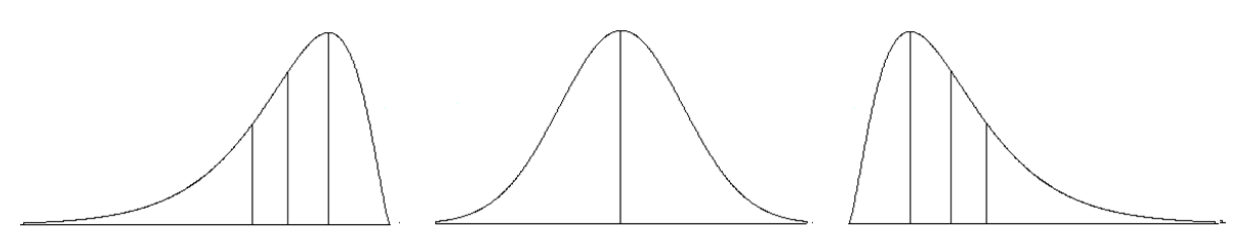
\includegraphics[width=1\textwidth]{skewness.png}
    \caption[Visual representation of skewness]{Visual representation of skewness. Removed from \cite{doi:10.1080/10691898.2011.11889611}}
    \label{fig:skewness}
  \end{center}
\end{figure}

The skewness of attributes is calculated through the Equation \ref{eq:skew}:

\begin{equation}
  \label{eq:skew}
  skewness_x=\frac{m_3}{sd_x^3}
\end{equation}

Where $sd_x^3$ and $m_3$ are extracted from the formulas \ref{eq:skew1} and \ref{eq:mj}.

\begin{equation}
  \label{eq:skew1}
  sd_x^3=\sqrt{\frac{\sum_{i=1}^{n}(x_i - \bar{x})^2}{n-1}}
\end{equation} 

\begin{equation}
  m_j=\frac{1}{n}\sum_{i=1}^{n}(x_i-\bar{x})^j
  \label{eq:mj}
\end{equation}

Applying skewness to the generation process can require only a tiny tweaking in dataset generators that already use a normal distribution to create synthetic datasets. Luckily, python's library script Skewnorm's function\footnote{\href{https://docs.scipy.org/doc/scipy/reference/generated/scipy.stats.skewnorm.html}{docs.scipy.org/}} had the required functions that allowed us to perform our experimentation. This function takes a number as a skewness parameter. When that number equals 0, the distribution is identical to a normal distribution.

In Listing \ref{lst:skew} we display the used code to perform the insertion of a skewness of value -2 into a normal distribution.

\begin{lstlisting}[language=Python, caption=Integrating skewness, label={lst:skew}]
NumValues = 10000
maxValue = 6
skewness = -2 

random = skewnorm.rvs(a=skewness, loc=maxValue, size=numValues)

random = random - min(random)
random = random / max(random)
random = random * maxValue 
\end{lstlisting}

\begin{figure}[!ht]
    \centering
    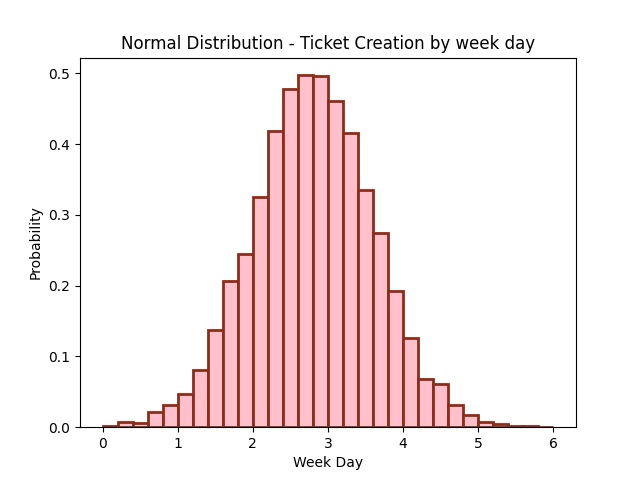
\includegraphics[width=.45\textwidth]{myplot_normal.jpg}
    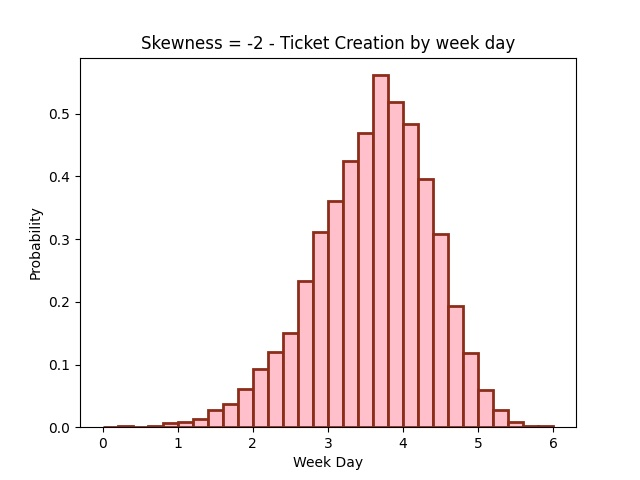
\includegraphics[width=.45\textwidth]{myplot_sk-2.jpg}
    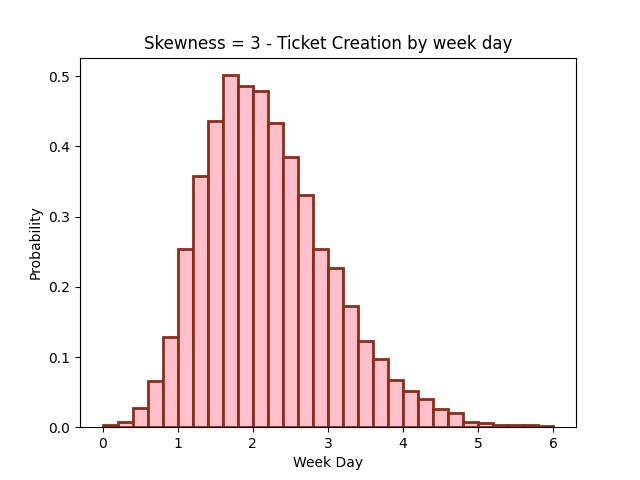
\includegraphics[width=.45\textwidth]{myplot_sk3.jpg}
    \caption{Skewness integration}
    \label{fig:skew-int}
\end{figure}

We could then move on to experimentation. Using a normal distribution, we studied the distribution of 10000 tickets generated by day of the week (0 being Sunday and 6 Saturday). We tried to influence the distribution probability by inputting a skewness value.

The results of this testing can be seen in Figure \ref{fig:skew-int}. We started by creating a normal distribution that had a skewness of 0. We changed that value to -2 and 3 and exported the end results in graphical form.

Having these outcomes, we can conclude that we can indeed generate a synthetic dataset with a chosen value of kurtosis by influencing the probability distribution of values in the generator.





%To generate skewness to either side, we just need to ensure that the mean value stays the same as it would on standard generation while shifting the mode and median to the other side. This is done by generating an extensive but focused amount of values on the opposite side of the skew while creating a spread-out number of entries on the side of the skew, generating a skewness tail on the desired side of the aisle.
\subsection{Kurtosis}

Kurtosis is a "measure of the "tailedness" of the probability distribution of a real-valued random variable" (adapted from \cite{ramya2017breast}). Like skewness, kurtosis describes the shape of a probability distribution. There are different ways of quantifying it for a theoretical distribution and corresponding ways of estimating it from a sample from a population. Other measures of kurtosis may have varied interpretations. As \cite{doi:10.1080/00031305.1988.10475539} said, and I quote: "It is best to define kurtosis vaguely as the location- and scale-free movement of probability mass from the shoulders of a distribution into its center and tails and to recognize that it can be formalized in many ways."

Kurtosis is sometimes confused with a measure of the peakedness of a distribution \citep{doi:10.1080/00031305.1970.10478885}. However, kurtosis is a measure that describes the shape of a distribution's tails concerning its overall format. All kurtosis measures are analogized against a typical normal distribution or bell curve.

\begin{figure}[!ht]
  \begin{center}
    \leavevmode
    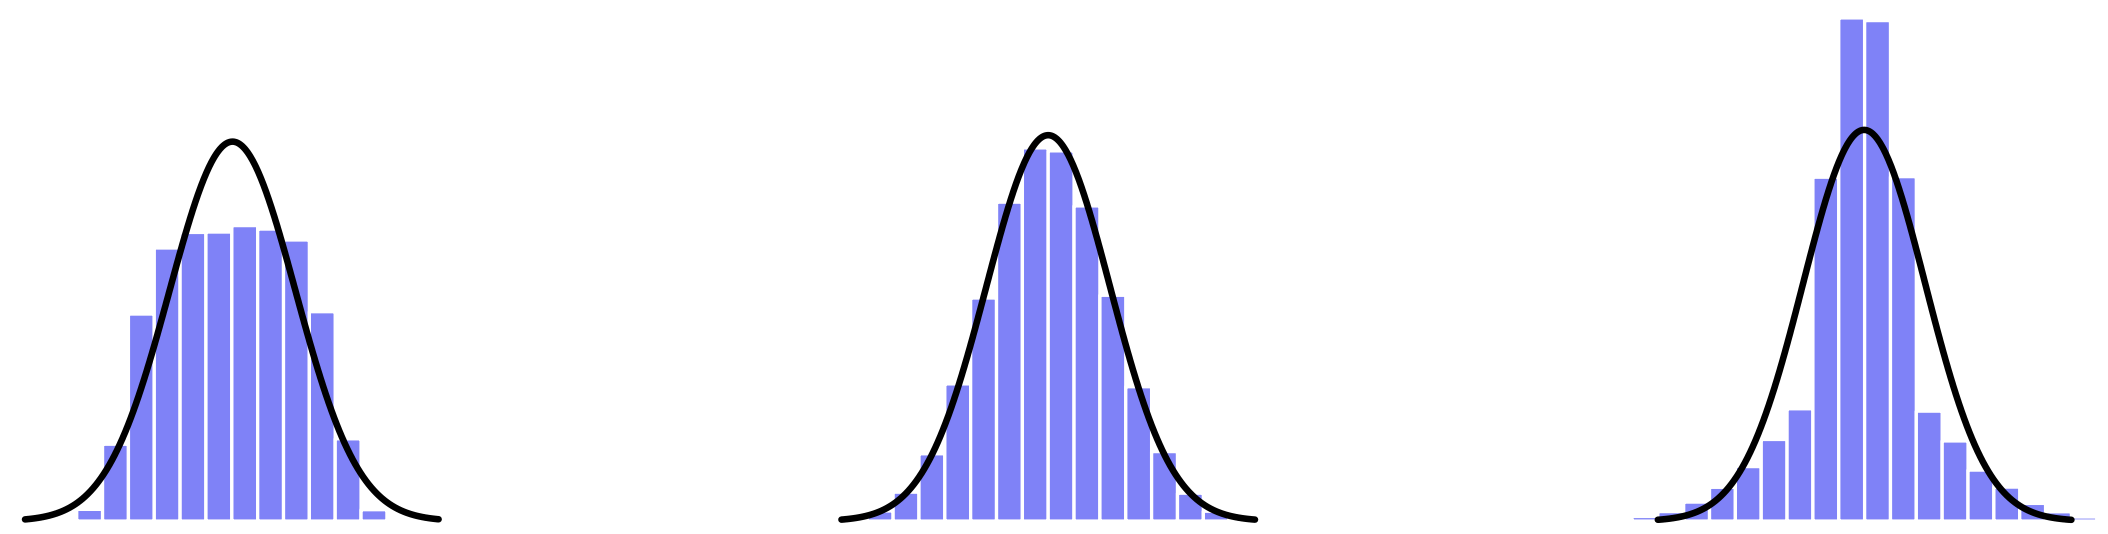
\includegraphics[width=1\textwidth]{kurtosis_histogram.png}
    \caption[Visual representation of kurtosis in histogram form]{Visual representation of kurtosis in histogram form. Removed from \cite{navarro2019learning}}
    \label{fig:kurtosis}
  \end{center}
\end{figure}

As depicted in Fig. \ref{fig:kurtosis} kurtosis can be represented in 3 types. The left graph is called a platykurtic distribution. These distributions have short tails with flattened curves. The middle graph represents a mesokurtic kurtosis distribution where kurtosis is almost exactly 0. Finally, on the right, we have a leptokurtic kurtosis, where the values of the normal distribution peak. The modal curve represented by a black curve in the figure has a kurtosis value equal to 0.

Kurtosis can be calculated using the formula \ref{eq:kurt}.
\begin{equation}
  \label{eq:kurt}
  kurt_x=\frac{m_4}{sd_x^4}-3
\end{equation}

Where $m_4$ is calculated using the formula presented in Equation \ref{eq:mj}

As with Skewness integration, adding desired kurtosis values could be done by changing the parameters of the output entries. However, influencing this value is not as easy as initially thought. Using a simple value of Kurtosis was not possible. However, we could try using different distributions and see how their Kurtosis values would influence the shape of the output dataset.
%For negative skewness, we need to reduce the number of entries closer to the mean of the distribution while assuring that output continues to be a normal distribution (only flattened in comparison to the original). Positive skewness would do the inverse, increasing the production of entries closer to the mean, creating a peak of values.

\begin{figure}[!ht]
    \centering
    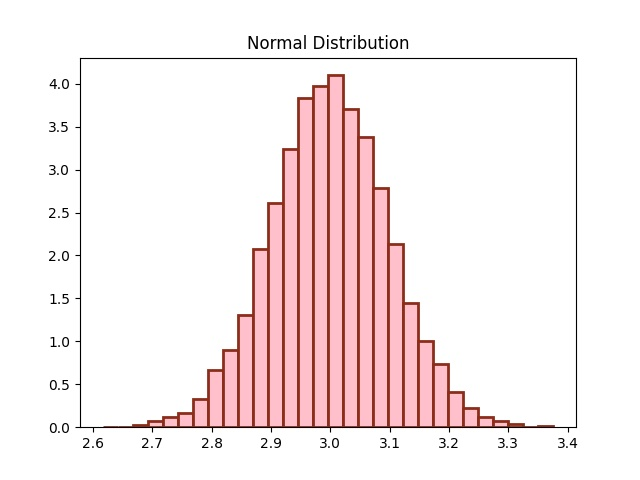
\includegraphics[width=.45\textwidth]{normal.jpg}
    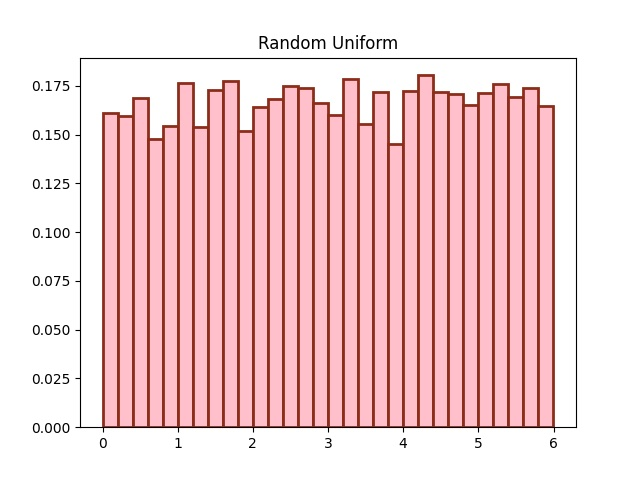
\includegraphics[width=.45\textwidth]{uniform.jpg}
    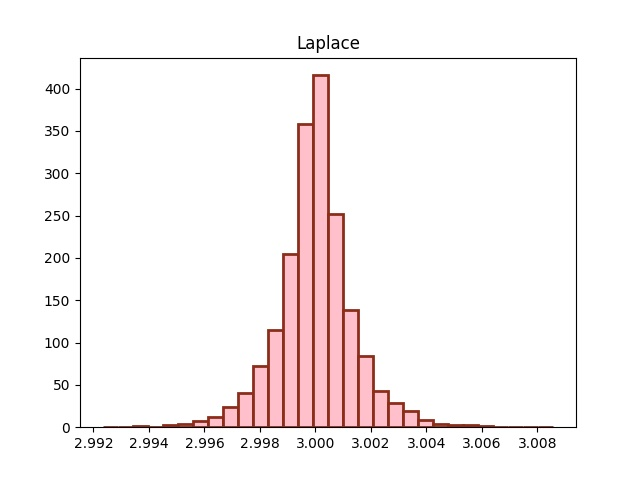
\includegraphics[width=.45\textwidth]{laplace.jpg}
    \caption{Normal, Random Uniform and Laplace distributions}
    \label{fig:kurt-int}
\end{figure}

\pagebreak
Results of this testing can be seen in Figure \ref{fig:kurt-int}. We used different distributions to generate data with distinguishable characteristics. We then calculated kurtosis on these distributions and see if its values changed according to the distribution. The uniform distribution had a kurtosis value of 1.8, Normal distribution had a value of 3. Finally, with Laplace, we arrived at a kurtosis value of 6.59.

While we found that it is possible to influence the value of kurtosis we found to way of correctly influencing that same value with a simple user input.
\section{Information-theoretic}
Information-theoretic meta features are based on entropy, capturing the data's amount of information and complexity. 
The entropy ($H_{x}$) can be given by the formula \ref{eq:if}.
\begin{equation}
  \label{eq:if}
  H_{x}=-\sum_{x=1}^{N}P_{x}log_{2}(P_{x})
\end{equation}
Where $P_{x}$ represents the probability of a category (x) to occur.

We can use this formula to calculate certain meta features in this family, such is the case of the classEnt meta feature.

Solving this problem to force a specific entropy value is a mathematical one that exceeds our capabilities. Nevertheless, from an engineering standpoint, we propose the analysis of entropy at set intervals during the generation process. For each gap, we would freeze the generation, calculate entropy and see how far we are from our target. In cases where values are superior to the desired ones, we should try to generate more noise, reducing the more significant percentages and lowering the entropy. In cases where we were already lower, we should focus the generation on existing, more probable values. This would increase their final probability and levelling our entropy values. 

Would setting a particular value of entropy be helpful to the final dataset? In a simple answer, yes. Entropy measures disorder or impurities in the information processed in machine learning. The ability to choose that purity level has obvious benefits from an ML study standpoint.

\section{Landmarking}
We arrived at strange conclusions regarding landmarking meta features when analysing possible meta features to validate their inclusion in synthetic dataset generation processes. These meta features use algorithms to characterise datasets. To include specific values of these meta features, we would need to create entries while also knowing how well the entire dataset would behave when fronting said algorithm.

A funny analogy to this problem would be to drive a train while building the train tracks, taking into account the performance of every vehicle on the railroad system. The complexity of this problem vastly overshadows the scope of this study.

Landmarking inclusion would be rather valuable, especially in machine learning cases. Users could generate datasets with good and bad results, teaching the MLM to follow datasets with good results. However, their inclusion could prove troublesome as data could serve the dataset too perfectly. 

Generating datasets with set algorithmic results would lead to synthetic datasets riddled with overfitting problems.

\section{Dataset Morphing}
One option we came across to use to create datasets with specific values of meta features was dataset morphing. With dataset morphing, we could change it after having a complete dataset and altering its values to achieve the desired meta feature value results.

This, however, comes with a set of problems. Let's use the same case we already used with kurtosis and skewness. So we want to alter the ticket generation time by day of the week. To do this, we need to finish the generation process and then change the data on columns related to that information. This change also needs to impact the rest of the dataset, not just that one column. The generation process would need to be halted in columns whose data depends on the morphed columns. Only after the data connected to the morphing finishes being generated and is morphed can the generation process continue.

This process is more time and resource expensive than normal run-time generation.
\section{Conclusion}
In this chapter, we looked at the original approach taken to test some of the methodologies later described in the chapter. 

We then analysed some possible meta feature inclusions to the generation process. We explored the possibility of including general, statistical, information-theoretic and landmarking meta features. We also looked at the validity of incorporating these meta features in each analysis.

We also looked at the possibility of dataset morphing to insert meta feature values into a synthetic dataset.

While we found it possible to insert meta features, we did it in a singular factor. By inserting a meta feature, we cannot guarantee that the values of other meta features in the dataset will be maintained.

Datasets generated with dataset integration, be it by runtime integration or morphing should them be analysed to see if they continue to be valid and realistic. A debugging analysis should be made, in order to guarantee the stability of buisiness rules inside the dataset to guarantee the validity of the data. Some of the data evaluation methods described in Chapter \ref{chap:generation} should also be used to check the validity of the final output.

When looking at what was achieved in this part of the study and what was initially idealised, it is impossible not to feel underwhelmed. We analysed ways to force certain meta features into the generation process. We proved that this implementation can be done on simple and statistical meta features. We conclude that a complete study on the subject should be made to get to any plausible conclusion on including meta features with more complicated calculations.